\documentclass[a4paper]{article}


\usepackage[T1]{fontenc}
\usepackage[utf8]{inputenc}
\usepackage{mathptmx}

%\usepackage{ngerman}	% Sprachanpassung Deutsch

\usepackage{graphicx}
\usepackage{geometry}
\geometry{a4paper, top=15mm}

\usepackage{subcaption}
\usepackage[shortlabels]{enumitem}
\usepackage{amssymb}
\usepackage{amsthm}
\usepackage{mathtools}
\usepackage{braket}
\usepackage{bbm}
\usepackage{graphicx}
\usepackage{float}
\usepackage{yhmath}
\usepackage{tikz}
\usetikzlibrary{patterns,decorations.pathmorphing,positioning}
\usetikzlibrary{calc,decorations.markings}

\usepackage[backend=biber, sorting=none]{biblatex}
\addbibresource{uni.bib}

\usepackage[framemethod=TikZ]{mdframed}

\tikzstyle{titlered} =
    [draw=black, thick, fill=white,%
        text=black, rectangle,
        right, minimum height=.7cm]


\usepackage[colorlinks=true,naturalnames=true,plainpages=false,pdfpagelabels=true]{hyperref}
\usepackage[parfill]{parskip}
\usepackage{lipsum}


\usepackage{tcolorbox}
\tcbuselibrary{skins,breakable}

\pagestyle{myheadings}

\markright{Popović\hfill Tensor Methods \hfill}


\title{University of Vienna\\ Faculty of Mathematics\\
\vspace{1cm}TENSOR METHODS FOR DATA SCIENCE AND SCIENTIFIC COMPUTING
}
\author{Milutin Popovic}

\begin{document}
\maketitle
\tableofcontents
\section{Assignment 3}
\subsection{Implementing the CP-ALS Algorithm}
The main idea of the algorithm is that we have a rank $R\in \mathbb{N}$ CPD
of a tensor $A \in \mathbb{R}^{n_1 \times \cdot n_d}$ given in terms of
$U_k \in \mathbb{R}^{n_k \times R}$, for $\mathbb{N}\ni k>2$, $k =
\{1,\dots,d\}$ and for $n_1, \dots, n_d\; \in \mathbb{N}$. We want to find a
rank $r\in \mathbb{N}$ CPD of the tensor $A$, by taking an initial guess
for some $V_k \in \mathbb{R}^{n_k \times r}$ and updating it for each $k$ by
optimizing the problem
\begin{align}
    \phi(V_1, \dots, V_d) \rightarrow \min_{V_k \in \mathbb{R}^{n_k\times
    r}},
\end{align}
where $\phi(V_1, \dots, V_d)$ is the error function, determined by
\begin{align}
    \phi(V_1, \dots, V_d) = \left\|\Psi_r(V_1,\dots,V_d) - \Psi_R(U_1,
    \dots,U_d) \right\|_F .
\end{align}
For $\Psi_r$ and $\Psi_R$ denote the CPD multilinear representation maps
transforming the CP decomposition into the tensor
\begin{align}
    U &= \Psi_R(U_1, \dots, U_d)\\
    V &= \Psi_r(V_1, \dots, V_d)\\
 \end{align}
for $k = 1, \dots d, d-1, \dots 2$ sequentially by updating $V_k$ at each
step of the optimization. \textbf{This is one iteration step}.

For $\Psi$ we will use the implementation constructed in the last exercise,
which consists of applying the Kronecker product of the rows and then
summing over them. Once we define the following matrices we may rewrite the
optimality condition in a linear system which is solvable since it is a least
square problem. We define matrices $\mathcal{V}_k \in \mathbb{R}^{n_1\cdots n_d
\times n_k\cdot r}$ and $\mathcal{U}_k \in \mathbb{R}^{n_1\cdots n_d \times
n_k\cdot R}$ for $k \in \{1, \dots,d\}$  by the following
\begin{align}
    \mathcal{U}_k &= \prod_{\substack{l=1 \\ l!=k}}^{d} U_l \otimes
    \mathbbm{1}_{\mathbb{R}^{n_k\times n_k}},\\
    \mathcal{V}_k &= \prod_{\substack{l=1 \\ l!=k}}^{d} V_l \otimes
    \mathbbm{1}_{\mathbb{R}^{n_k\times n_k}},
\end{align}
note that $\prod$ represents the Hadamard product (elementwise multiplication) and
$\otimes$ the Kronecker product. The product of these two new defined
matrices is then simply
\begin{align}
    \mathcal{V}_k^*\mathcal{V}_k &=  \prod_{\substack{l=1 \\ l!=k}}^{d}
    (V_l^*V_l) \otimes \mathbbm{1}_{\mathbb{R}^{n_k\times n_k}}
    \label{eq: VV}    \\
    \mathcal{V}_k^*\mathcal{U}_k &=  \prod_{\substack{l=1 \\ l!=k}}^{d}
    (V_l^*U_l) \otimes \mathbbm{1}_{\mathbb{R}^{n_k\times n_k}}.\label{eq:
        VU}
\end{align}
Do note that $\mathcal{V}_k^*\mathcal{V}_k \in \mathbb{R}^{r\cdot n_k \times
r\cdot n_k}$ and $\mathcal{V}_k^*\mathcal{U}_k \in \mathbb{R}^{r\cdot n_k
\times R\cdot n_k}$. For convenience let us define $F_k := V_k^* U_k$ and
$G_k := V_k^* V_k$, which will become useful when talking about storing the
computation. The we can solve for $V_k$ with the following least square
problem
\begin{align}
    (\mathcal{V}_k^*\mathcal{V}_k)\hat{v}_k = (\mathcal{V}_k^*\mathcal{U}_k)u_k,
\end{align}
where $\hat{v}_k = \text{vec}(\hat{V}_k)$ and $u_k = \text{vec}(U_k)$.

To make the computation cost linear with respect to $d$, we can compute
$\mathcal{V}_k^*\mathcal{V}_k$ and $\mathcal{V}_k^*\mathcal{U}_k$ for
each $k$ and update them in the iteration in $k$ with the new $\hat{V}_k$, by
computing the product in equations \ref{eq: VV} and \ref{eq: VU} again.
Additionally we compute the error $\phi$ and $\|\nabla \frac{1}{2}
\phi^2\|_2$ after each iteration (after going through
$k=2,\dots,d,d-1,\dots,1$). The implementation is in \cite{code}.

\subsection{CP-ALS for the matrix multiplication tensor}
In this section we will use the matrix multiplication tensor to play around
the CP-ALS algorithm we implemented in the last section. We consider $n = 2$
and $r = 7$, $n = 3$ and $r = 23$, $n = 4$ and $r = 49$ for the
multiplication tensor and its CP decomposition. The implementation of them we
have done in the last exercise together with their rank $R = n^3$ CP
decomposition. We test the our implementation of the CP-ALS algorithm of
these three multiplication tensor for three random initial guesses $V_1, V_2,
V_3$, where each matrix has unitary columns (i.e. of norm one).

Our procedure will be that we do seven different guesses if they are good
enough, i.e. if they do not produce a \textit{SingularValueError} after 10
iterations we go for 10000 iterations and plot both $\phi$ and $\|\nabla
\frac{1}{2} \phi\|_2$ with respect to the number of iterations for each
multiplication tensor. We get the following curves
\begin{figure}[H]
    \centering 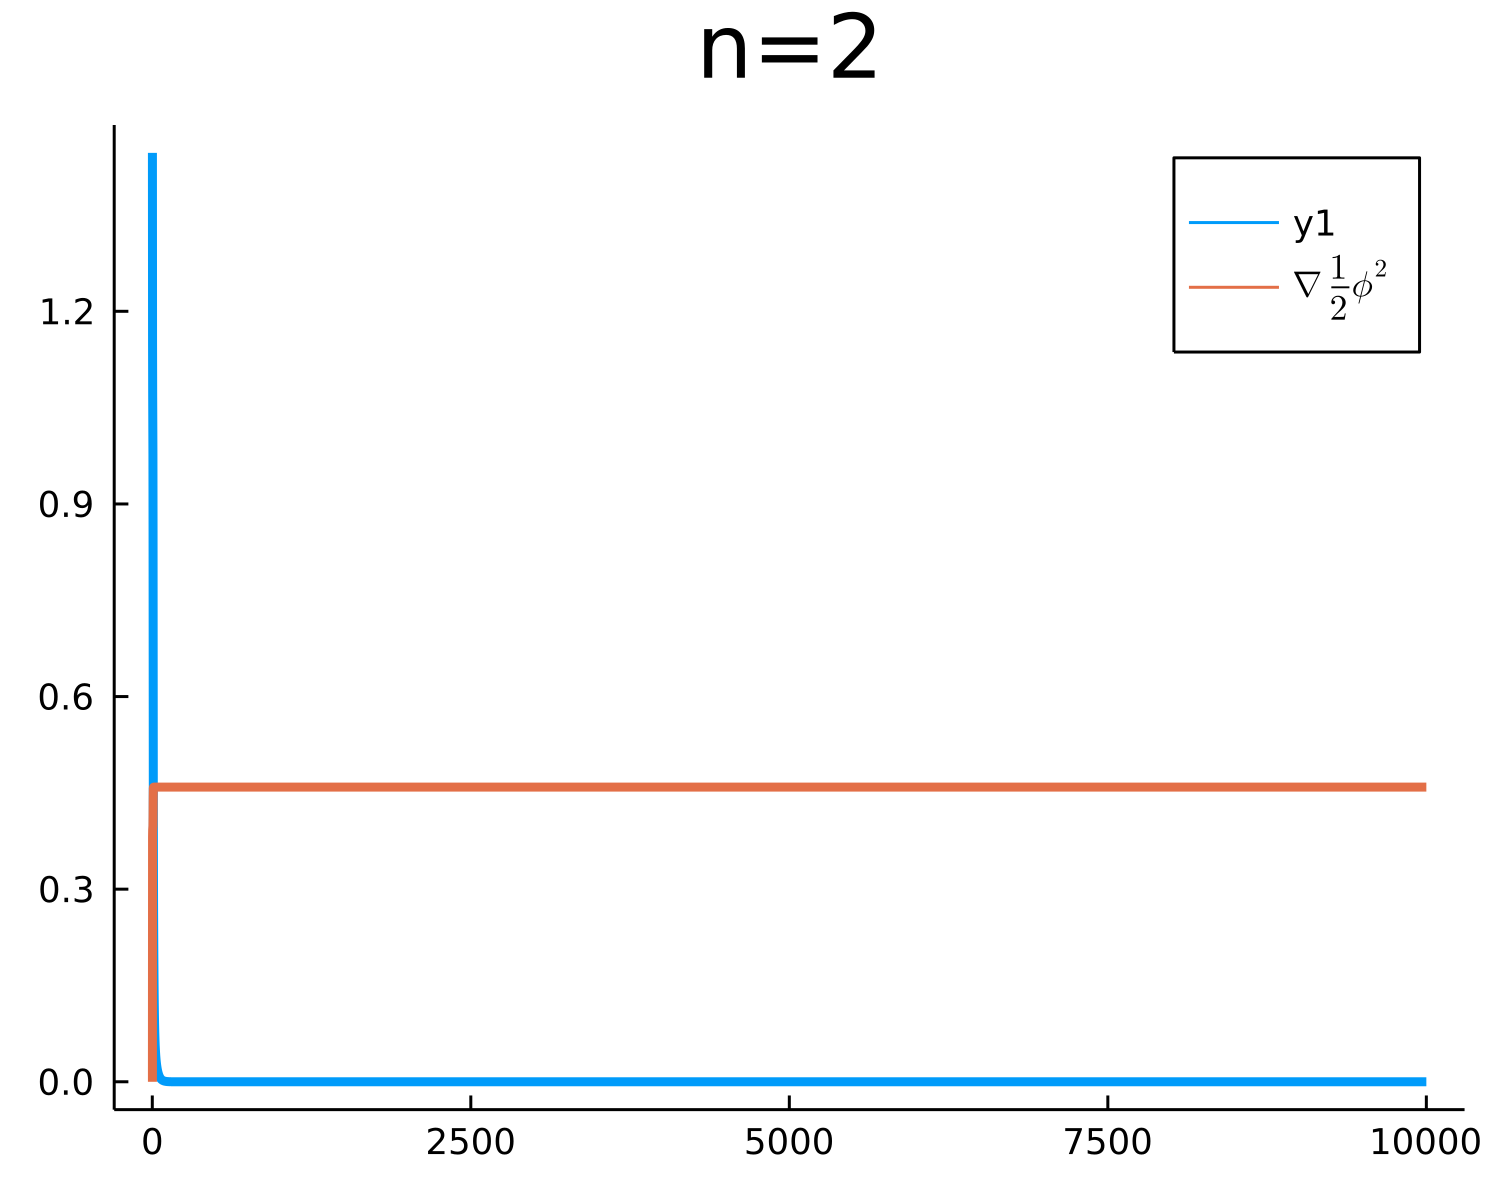
\includegraphics[width=0.33\textwidth]{./../src/plots/err_2.png}
    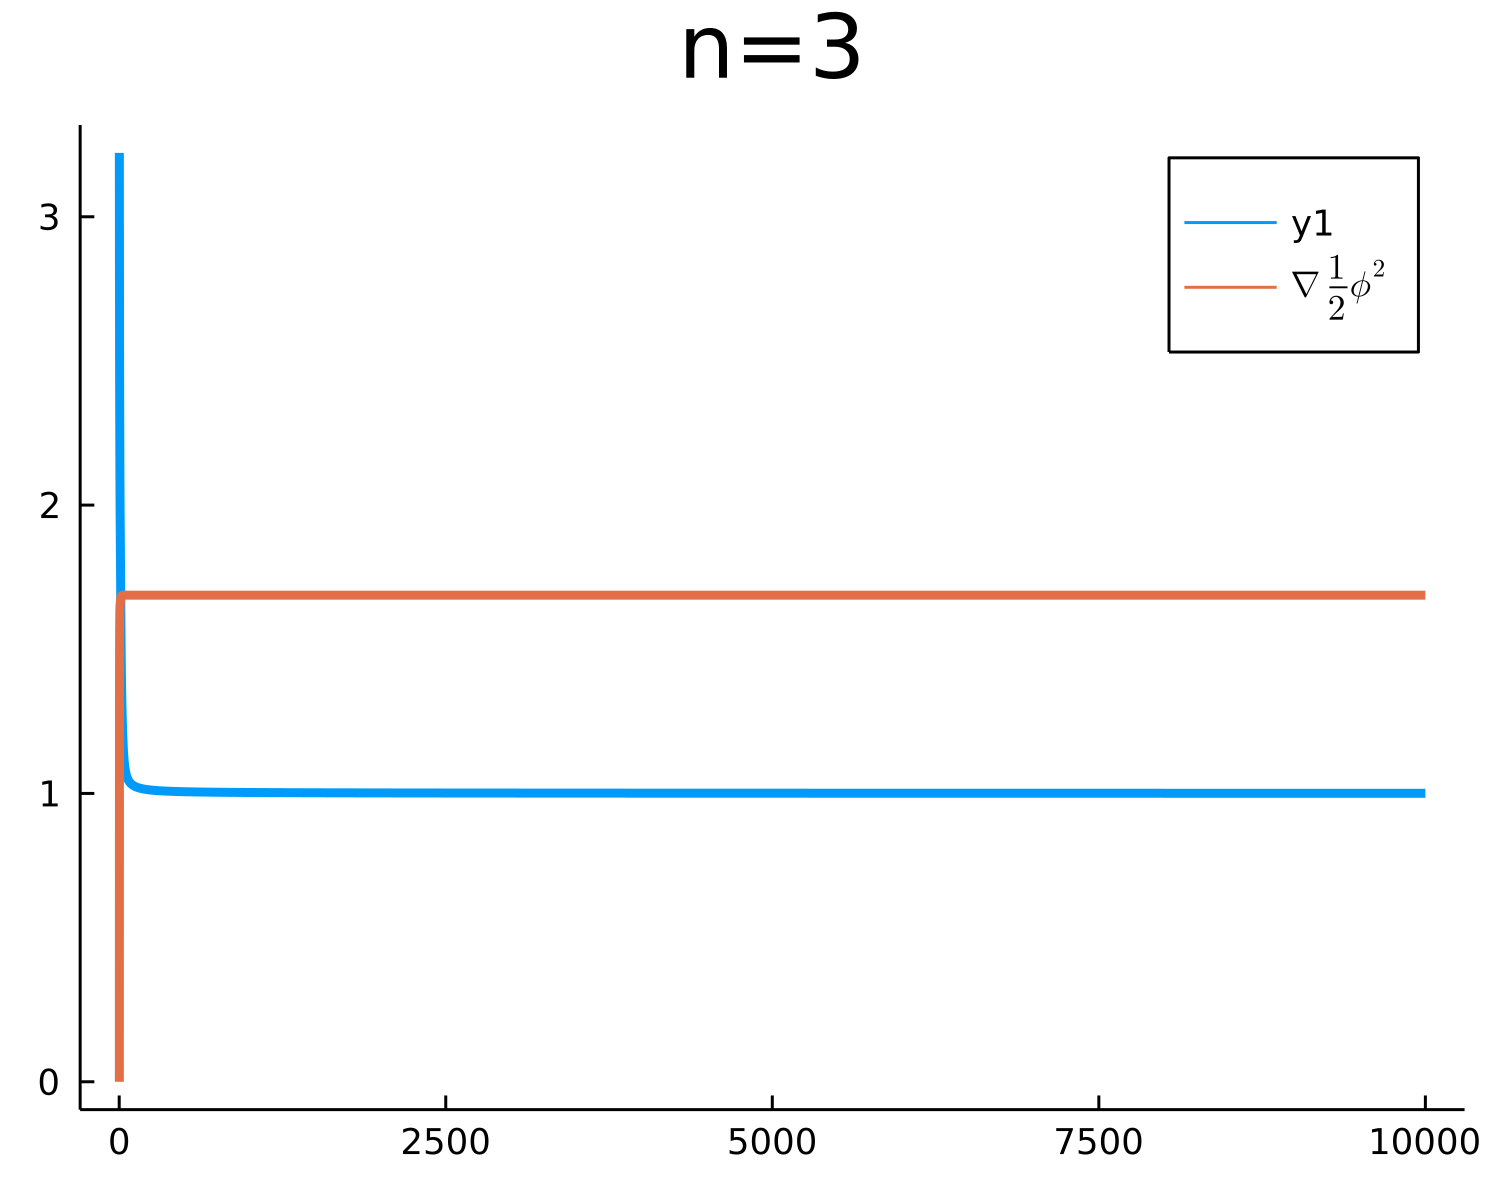
\includegraphics[width=0.33\textwidth]{./../src/plots/err_3.png}
    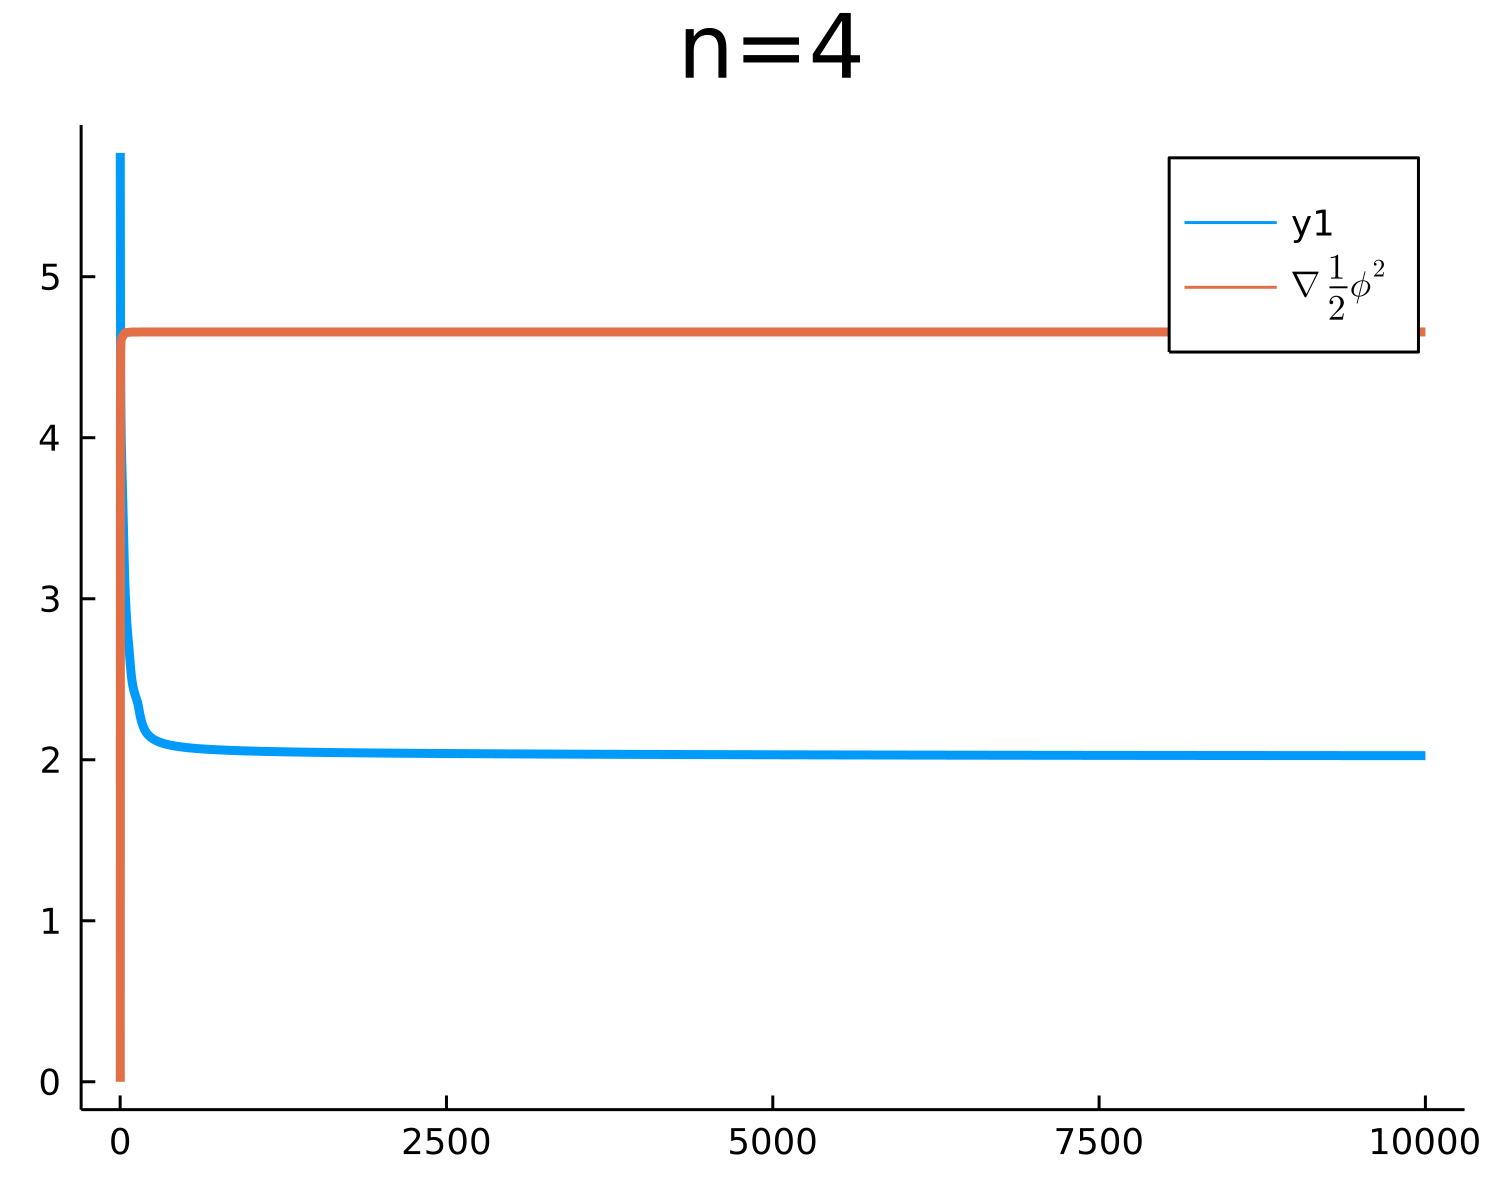
\includegraphics[width=0.32\textwidth]{./../src/plots/err_4.png}
    \caption{From left to right, rank $r\in\{7, 23, 49\}$ CP-ALS error for the
    $n\in \{2, 3, 4\}$ multiplication tensor at 10000 iteration steps}
\end{figure}



\printbibliography
\end{document}
